{A solid with length 10 with a rectangular base and triangular top, wherein one end is a square with side length 5 and the other end is a triangle with base and height of 5.

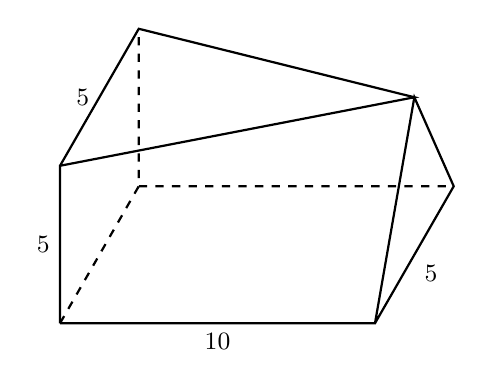
\begin{tikzpicture}[x={(1,0)},z={(0,1)},y={(.5,.87)},scale=.4]

\draw [thick] (0,0,0) -- node[pos=.5,below] {\small 10} (10,0,0) -- (10,2.5,5) -- (10,5,0) -- node [pos=.5,below right] {\small 5} (10,0,0)
							(0,0,0) -- node [pos=.5,left] {\small 5} (0,0,5) -- (10,2.5,5) -- (0,5,5) -- node [pos=.5,left] {\small 5} (0,0,5);
							
\draw [thick,dashed] (0,0,0) -- (0,5,0) -- (0,5,5)
										(0,5,0) -- (10,5,0);



\end{tikzpicture}}
{Orient the solid so that the $x$-axis is parallel to long side of the base. All cross--sections are trapezoids (at the far left, the trapezoid is a square; at the far right, the trapezoid has a top length of 0, making it a triangle). The area of the trapezoid at $x$ is $A(x) = 1/2(-1/2x+5+5)(5) = -5/4x+25$. The volume is $187.5$ units$^3$.
}
